\documentclass[12pt,a4paper]{article}
\usepackage[utf8]{inputenc}
\usepackage[ngerman]{babel}
\usepackage{geometry}
\usepackage{fancyhdr}
\usepackage{graphicx}
\AtBeginDocument{\graphicspath{{images/}}}
\usepackage{amsmath}
\usepackage{amsfonts}
\usepackage{amssymb}
\usepackage{listings}
\usepackage{listingsutf8}
\lstset{inputencoding=utf8,
extendedchars=true}
\lstset{literate=%
{Ü}{{\"U}}1
{ü}{{\"u}}1
{ä}{{\"a}}1
{ö}{{\"o}}1
{Ä}{{\"A}}1
{Ö}{{\"O}}1
{ß}{{\ss}}2}
\lstset{escapeinside={§}{§}}
\usepackage{xcolor}
\usepackage{hyperref}
\usepackage{tocloft}
\usepackage{float}
\usepackage{subcaption}
\usepackage{booktabs}
\usepackage{algorithm}
\usepackage{algorithmic}

% Seitenränder
\geometry{left=3cm,right=2.5cm,top=3cm,bottom=3cm}

% Kopf- und Fußzeilen
\pagestyle{fancy}
\fancyhf{}
\fancyhead[L]{\leftmark}
\fancyhead[R]{\thepage}
\renewcommand{\headrulewidth}{0.4pt}

% Python Code Highlighting
\lstdefinestyle{pythonstyle}{
    language=Python,
    backgroundcolor=\color{gray!10},
    commentstyle=\color{green!60!black},
    keywordstyle=\color{blue},
    numberstyle=\tiny\color{gray},
    stringstyle=\color{red!80!black},
    basicstyle=\footnotesize\ttfamily,
    breakatwhitespace=false,
    breaklines=true,
    captionpos=b,
    keepspaces=true,
    numbers=left,
    numbersep=5pt,
    showspaces=false,
    showstringspaces=false,
    showtabs=false,
    tabsize=2,
    frame=single,
    rulecolor=\color{black!30}
}
\lstset{style=pythonstyle}

% Hyperlink Setup
\hypersetup{
    colorlinks=true,
    linkcolor=blue,
    filecolor=magenta,
    urlcolor=cyan,
    citecolor=green,
    pdfinfo={
        Title={Intelligente Pfadsuche: Vergleichende Simulation von Suchverfahren in generierten Maze-Umgebungen},
        Author={Ihr Name},
        Subject={Angewandte Modellierung Endprojekt},
    }
}

\begin{document}

% ================== DECKBLATT ==================
\begin{titlepage}
    \centering
    \vspace*{2cm}
    
    {\LARGE\textbf{BTU Cottbus-Senftenberg}}\\[0.5cm]
    {\Large Fachbereich Drahtlose Systeme}\\[2cm]
    
    {\huge\textbf{Intelligente Pfadsuche}}\\[0.5cm]
    {\LARGE\textbf{Vergleichende Simulation von Suchverfahren in generierten Maze-Umgebungen}}\\[3cm]
    
    {\Large Endprojekt im Rahmen der Vorlesung}\\[0.3cm]
    {\Large\textbf{Angewandte Modellierung und Systemsimulation}}\\[2cm]
    
    \begin{tabular}{ll}
        \textbf{Autor:} & Ole Matzky\\[0.3cm]
        \textbf{Matrikelnummer:} & 5005801 \\[0.3cm]
        \textbf{Studiengang:} & Künstliche Intelligenz \\[0.3cm]
        \textbf{Semester:} & 4. Semester \\[0.3cm]
        \textbf{Betreuer:} & Dr. Svetlana Meissner \\[0.3cm]
        \textbf{Abgabedatum:} & 22. Juli 2025 \\
    \end{tabular}
    
    \vfill
    
    {\large\today}
\end{titlepage}

% ================== INHALTSVERZEICHNIS ==================
\tableofcontents
\newpage

% ================== EINLEITUNG ==================
\section{Einleitung}

Die Pfadsuche in komplexen Umgebungen ist ein fundamentales Problem der Informatik mit weitreichenden Anwendungen in der Robotik, Spieleentwicklung und Navigationssystemen. Dieses Projekt implementiert eine interaktive Visualisierung verschiedener Pathfinding-Algorithmen in zufällig generierten Labyrinthen.

Das entwickelte System ermöglicht es, drei klassische Suchalgorithmen -- A*, Dijkstra und Greedy Best-First Search -- in ihrer Funktionsweise zu vergleichen und deren charakteristische Eigenschaften durch animierte Visualisierungen zu verstehen.

\subsection{Projektziele}
\begin{itemize}
    \item Implementierung eines Maze-Generators basierend auf randomisierter Tiefensuche
    \item Entwicklung einer benutzerfreundlichen grafischen Oberfläche
    \item Vergleichende Analyse verschiedener Pathfinding-Algorithmen
    \item Bereitstellung von Exportfunktionalität für Animationen
\end{itemize}

% ================== MAZE-GENERIERUNG ==================
\section{Maze-Generierung}

\subsection{Randomisierte Tiefensuche}

Die Generierung der Labyrinthe erfolgt mittels einer randomisierten Tiefensuche (Randomized Depth-First Search). Dieser Algorithmus erzeugt garantiert ein \textit{perfektes Labyrinth}, das folgende Eigenschaften aufweist:

\begin{itemize}
    \item \textbf{Zusammenhängend}: Jede freie Zelle ist von jeder anderen freien Zelle aus erreichbar
    \item \textbf{Azyklisch}: Es existiert genau ein Pfad zwischen zwei beliebigen Punkten
    \item \textbf{Minimal}: Das Labyrinth enthält keine redundanten Verbindungen
\end{itemize}

\begin{algorithm}[H]
\caption{Randomisierte Tiefensuche für Maze-Generierung}
\begin{algorithmic}[1]
\STATE Initialisiere Grid mit Wänden
\STATE Wähle zufällige Startposition (ungerade Koordinaten)
\STATE Markiere Startposition als Pfad
\STATE stack = [Startposition]
\WHILE{stack nicht leer}
    \STATE current = stack.top()
    \STATE neighbors = unbesuchte Nachbarn von current (2 Schritte entfernt)
    \IF{neighbors existieren}
        \STATE next = zufälliger Nachbar aus neighbors
        \STATE Entferne Wand zwischen current und next
        \STATE Markiere next als besucht
        \STATE stack.push(next)
    \ELSE
        \STATE stack.pop()
    \ENDIF
\ENDWHILE
\end{algorithmic}
\end{algorithm}

\subsection{Ungerade Dimensionen und 2er-Schritte}

Die Verwendung ungerader Dimensionen und 2er-Schritte in der Tiefensuche ist essentiell für die korrekte Funktionsweise des Algorithmus:

\subsubsection{Ungerade Dimensionen}
\begin{itemize}
    \item Garantieren, dass Start- und Endpunkte auf gültigen Pfadpositionen liegen
    \item Vermeiden Randprobleme bei der Wandentfernung
    \item Stellen sicher, dass das resultierende Gitter die erforderliche Struktur aufweist
\end{itemize}

\subsubsection{2er-Schritte}
\begin{itemize}
    \item \textbf{Wanderhaltung}: Zwischen zwei Pfadzellen muss immer eine Wand liegen
    \item \textbf{Gitterstruktur}: Pfadzellen liegen nur auf ungeraden Koordinaten (1,1), (1,3), (3,1), etc.
    \item \textbf{Konnektivität}: Beim Überbrücken einer Wand werden genau zwei Schritte benötigt
\end{itemize}

\begin{figure}[H]
\centering
\begin{verbatim}
Beispiel 5x5 Grid:
W W W W W    # W = Wand, P = Pfad
W P W P W
W W W W W
W P W P W
W W W W W

Nach Verbindung von (1,1) zu (1,3):
W W W W W
W P P P W    # Wand bei (1,2) entfernt
W W W W W
W P W P W
W W W W W
\end{verbatim}
\caption{Gitterstruktur und Wandentfernung}
\end{figure}

\begin{figure}[H]
\centering
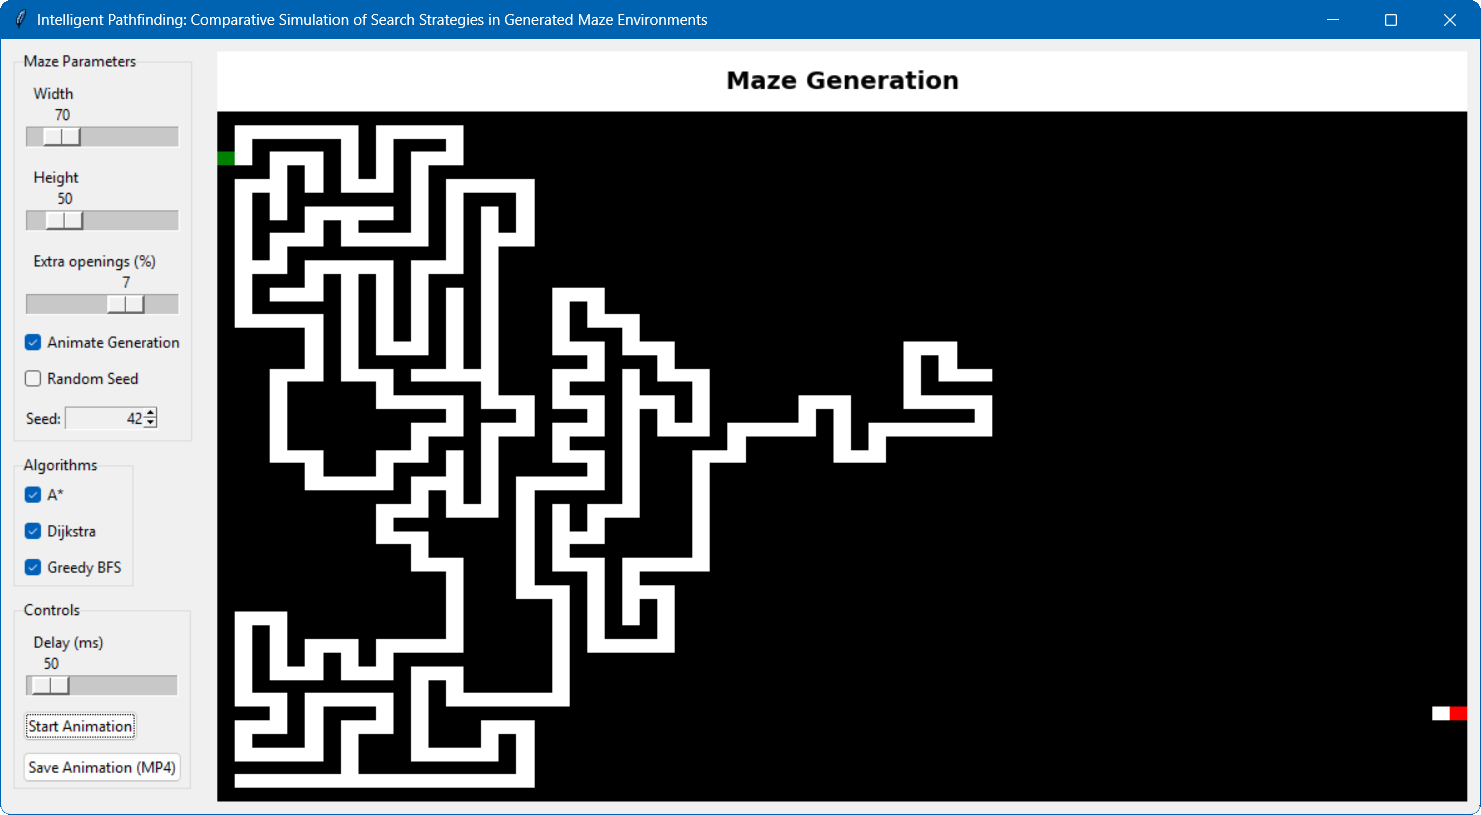
\includegraphics[width=\textwidth]{maze.png}
\caption{Maze-Generierung durch randomisierte Tiefensuche}
\label{fig:maze}
\end{figure}


\subsection{Datenrepräsentation als NumPy-Matrix}

Das Labyrinth wird als zweidimensionale NumPy-Matrix gespeichert, wobei jeder Zellenwert eine spezifische Bedeutung hat:

\begin{table}[H]
\centering
\begin{tabular}{cll}
\toprule
\textbf{Wert} & \textbf{Farbe} & \textbf{Bedeutung} \\
\midrule
0 & Weiß & Freier Pfad \\
1 & Schwarz & Wand \\
2 & Grün & Startposition \\
3 & Rot & Zielposition \\
4 & Gelb & Offene Knoten (in Queue) \\
5 & Hellblau & Aktueller Pfad \\
6 & Blau & Finaler optimaler Pfad \\
\bottomrule
\end{tabular}
\caption{Farbkodierung der Maze-Zellen}
\end{table}

\subsection{Reproduzierbarkeit durch Seed-Kontrolle}

Die Übergabe eines \texttt{numpy.random.Generator}-Objekts gewährleistet:

\begin{itemize}
    \item \textbf{Reproduzierbarkeit}: Identische Seeds erzeugen identische Labyrinthe
    \item \textbf{Testbarkeit}: Algorithmen können unter gleichen Bedingungen verglichen werden
    \item \textbf{Debugging}: Problematische Fälle können gezielt reproduziert werden
    \item \textbf{Wissenschaftlichkeit}: Experimente sind wiederholbar und verifizierbar
\end{itemize}

\begin{lstlisting}[caption={Beispiel für deterministische Maze-Generierung}]
from numpy.random import Generator, PCG64

# Deterministischer Generator
seed = 42
rng = Generator(PCG64(seed))

# Erzeugt immer das gleiche Labyrinth
maze = generator.generate_maze_grid(width, height, rng)
\end{lstlisting}

% ================== GENERATOR-PATTERN ==================
\section{Generator-Pattern und Lazy Evaluation}

\subsection{Python Generatoren}

Ein zentrales Designelement der Implementierung ist die extensive Nutzung von Python-Generatoren durch das \texttt{yield}-Keyword. Generatoren sind eine spezielle Art von Iteratoren, die Werte on-demand erzeugen.

\subsubsection{Was sind Generatoren?}

Generatoren sind Funktionen, die den Zustand zwischen Aufrufen beibehalten und Werte schrittweise produzieren:

\begin{lstlisting}[caption={Einfaches Generator-Beispiel}]
def simple_generator():
    print("Start")
    yield 1
    print("Zwischen den yields")
    yield 2
    print("Ende")

# Verwendung
gen = simple_generator()
print(next(gen))  # Output: "Start", dann 1
print(next(gen))  # Output: "Zwischen den yields", dann 2
\end{lstlisting}

\subsubsection{Vergleich mit bekannten Iteratoren}

Die \texttt{range()}-Funktion in Python 3 ist ein klassisches Beispiel für Lazy Evaluation:

\begin{lstlisting}[caption={Range als Iterator}]
# Erzeugt nicht alle Werte im Speicher
large_range = range(1000000)  # Sehr wenig Speicherverbrauch

# Versus Liste (Eager Evaluation)
large_list = list(range(1000000))  # Hoher Speicherverbrauch
\end{lstlisting}

\subsection{Vorteile der Generator-Nutzung}

\subsubsection{Speichereffizienz}
\begin{itemize}
    \item \textbf{Konstanter Speicherverbrauch}: Nur der aktuelle Frame wird gespeichert
    \item \textbf{Skalierbarkeit}: Funktioniert auch bei sehr großen Labyrinthen
    \item \textbf{Streaming}: Animationsframes werden just-in-time generiert
\end{itemize}

\subsubsection{Performance-Vorteile}
\begin{itemize}
    \item \textbf{Lazy Evaluation}: Berechnung nur bei Bedarf
    \item \textbf{Früher Ausstieg}: Animation kann jederzeit gestoppt werden
    \item \textbf{Pipeline-Verarbeitung}: Frames können direkt verarbeitet werden
\end{itemize}

% \begin{lstlisting}[caption={Generator für Maze-Animation}]
% def generate_maze_frames(self, width, height, rng, animate=True):
%     """Generator für Maze-Generierungs-Frames"""
%     # Initialisierung
%     grid = np.ones((height, width), dtype=int)
    
%     # Schrittweise Generierung
%     for step in self._dfs_steps(grid, rng):
%         if animate:
%             yield grid.copy()  # Nur bei Bedarf kopieren
    
%     # Sentinel-Wert für Ende
%     yield np.array([1])  # Signalisiert Fertigstellung
% \end{lstlisting}

% ================== GUI-FRAMEWORK ==================
\section{Grafische Benutzeroberfläche}

\subsection{Tkinter als GUI-Framework}

Die Wahl von Tkinter als GUI-Framework basiert auf mehreren Überlegungen:

\subsubsection{Persönliche Erfahrung}
\begin{itemize}
    \item Umfangreiche Erfahrung mit Tkinter in verschiedenen Projekten
    \item Vertrautheit mit Widgets und Layout-Management
\end{itemize}

\subsubsection{Community und Dokumentation}
\begin{itemize}
    \item \textbf{Hohe Popularität}: Weit verbreitet in der Python-Community
    \item \textbf{Umfangreiche Dokumentation}: Offizielle Docs und Community-Tutorials
    \item \textbf{Aktive Community}: Schnelle Hilfe bei Problemen
    \item \textbf{Stabilität}: Teil der Python-Standardbibliothek seit Python 1.0
\end{itemize}

\subsubsection{Widget-Prinzip}
Tkinter folgt dem bewährten Widget-Prinzip der GUI-Entwicklung:

\begin{lstlisting}[caption={Widget-Hierarchie in der Anwendung}]
class GUI(tk.Tk):  # Hauptfenster
    def __init__(self):
        # Container-Widgets
        main_container = tk.Frame(self)
        maze_config_frame = ttk.LabelFrame(parent_frame, text="Maze Parameters")
        
        # Input-Widgets  
        self.width_slider = tk.Scale(maze_config_frame, ...)
        self.height_slider = tk.Scale(maze_config_frame, ...)
        
        # Layout-Management
        maze_config_frame.pack()
        self.width_slider.grid(row=0, column=0, ...)
\end{lstlisting}

\subsection{Matplotlib-Integration}

\subsubsection{Warum Matplotlib für Animation?}

\begin{itemize}
    \item \textbf{Tkinter-Integration}: Nahtlose Einbettung via \texttt{FigureCanvasTkAgg}
    \item \textbf{Video-Export}: Direkte MP4-Exportfunktionalität
    \item \textbf{Professionelle Visualisierung}: Hochqualitative Grafiken
    \item \textbf{Animation-Framework}: \texttt{FuncAnimation} für flüssige Animationen
\end{itemize}

\begin{lstlisting}[caption={Matplotlib in Tkinter einbetten}]
def _setup_matplotlib_canvas(self):
    # Matplotlib Figure erstellen
    self.visualization_figure = plt.Figure(figsize=(10, 6))
    
    # In Tkinter einbetten
    self.matplotlib_canvas = FigureCanvasTkAgg(
        self.visualization_figure, master=self
    )
    self.matplotlib_canvas.get_tk_widget().grid(row=0, column=1)
    
    # Animation setup
    self.current_animation = FuncAnimation(
        self.visualization_figure, 
        self._update_frame,
        frames=self.frame_iterator,
        interval=50, blit=True
    )
\end{lstlisting}

\subsection{Steuerelemente der Benutzeroberfläche}

\subsubsection{Maze-Parameter}
\begin{itemize}
    \item \textbf{Width/Height Slider}: Kontrolle der Labyrinthgröße (30-300 × 20-200)
    \item \textbf{Extra Openings}: Zusätzliche Öffnungen für interessantere Pfade (0-10\%)
    \item \textbf{Animation Toggle}: Ein-/Ausschalten der Generierungs-Animation
    \item \textbf{Seed Control}: Deterministische vs. zufällige Generierung
\end{itemize}

\subsubsection{Algorithmus-Auswahl}
\begin{itemize}
    \item \textbf{Multi-Selection}: Mehrere Algorithmen gleichzeitig auswählbar
    \item \textbf{Sequential Execution}: Automatische Abarbeitung der gewählten Algorithmen
    \item \textbf{Live Comparison}: Echtzeit-Vergleich der Performance-Metriken
\end{itemize}

\subsubsection{Animation-Kontrolle}
\begin{itemize}
    \item \textbf{Delay-Slider}: Geschwindigkeitskontrolle (10-1000ms)
    \item \textbf{Export-Funktion}: MP4-Video-Export mit konfigurierbaren Optionen
\end{itemize}

\begin{figure}[H]
\centering
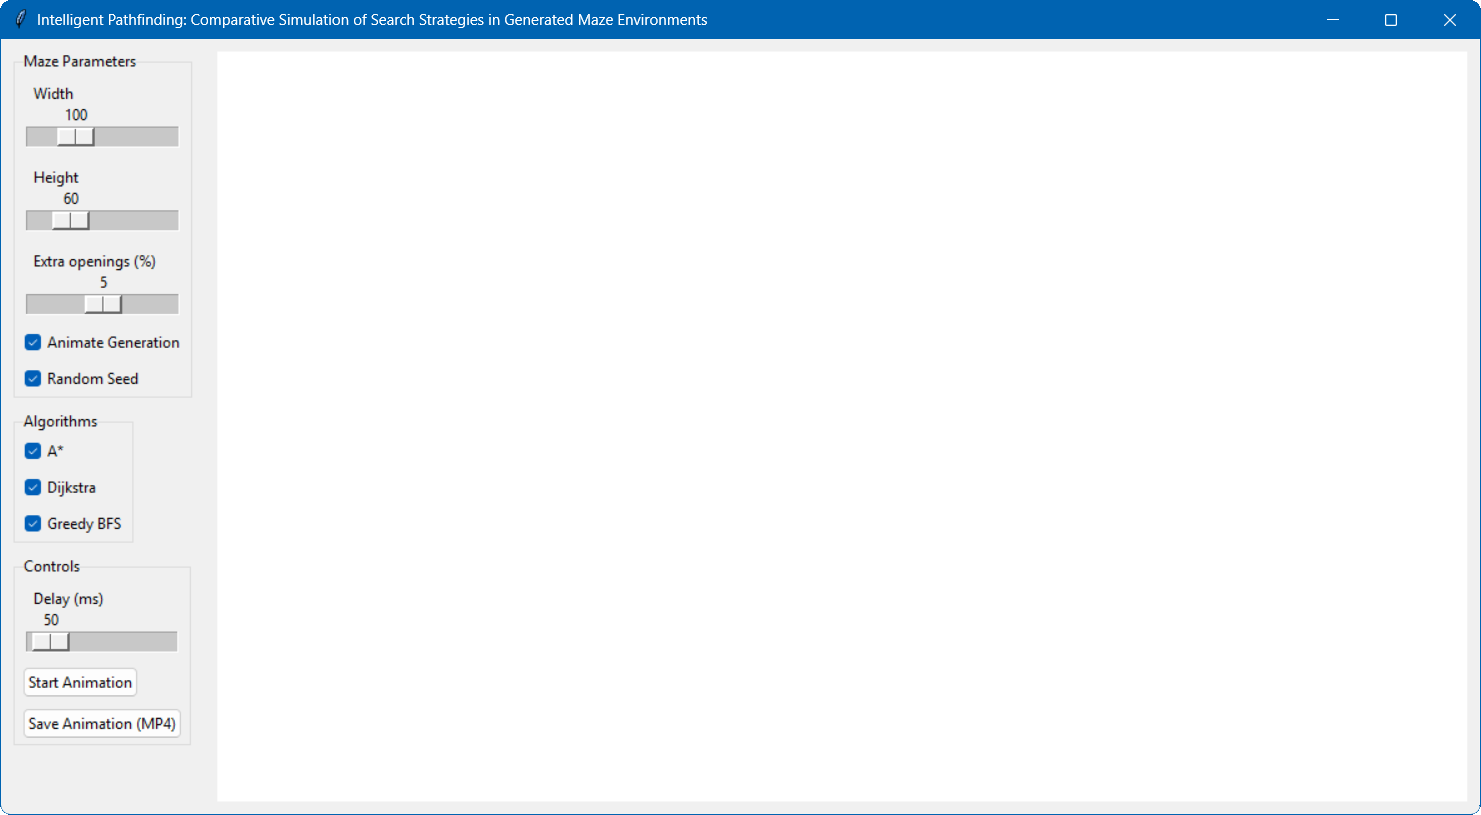
\includegraphics[width=\textwidth]{gui.png}
\caption{Benutzeroberfläche der Anwendung mit allen Steuerelementen}
\label{fig:gui}
\end{figure}

% ================== PATHFINDING-ALGORITHMEN ==================
\section{Pathfinding-Algorithmen}

\subsection{A* (A-Stern) Algorithmus}

A* ist ein informierter Suchalgorithmus, der eine Heuristik verwendet, um die Suche zu leiten.

\subsubsection{Funktionsweise}
\begin{itemize}
    \item \textbf{Bewertungsfunktion}: $f(n) = g(n) + h(n)$
    \item \textbf{Pfadkosten}: $g(n)$ = tatsächliche Kosten vom Start zu Knoten $n$
    \item \textbf{Heuristik}: $h(n)$ = geschätzte Kosten von $n$ zum Ziel
\end{itemize}

\subsubsection{Heuristik}
Verwendet Manhattan-Distanz: $h(n) = |x_n - x_{goal}| + |y_n - y_{goal}|$

\subsubsection{Eigenschaften}
\begin{itemize}
    \item \textbf{Optimal}: Findet den kürzesten Pfad (bei zulässiger Heuristik)
    \item \textbf{Vollständig}: Findet eine Lösung, wenn eine existiert
    \item \textbf{Effizient}: Deutlich schneller als uninformierte Suche
\end{itemize}

\subsection{Dijkstra-Algorithmus}

Dijkstra ist ein uninformierter Algorithmus, der alle Richtungen gleichmäßig erkundet.

\subsubsection{Funktionsweise}
\begin{itemize}
    \item \textbf{Bewertungsfunktion}: $f(n) = g(n)$ (nur Pfadkosten)
    \item \textbf{Strategie}: Erkundet Knoten in Reihenfolge der Pfadkosten
    \item \textbf{Garantie}: Findet immer den optimalen Pfad
\end{itemize}

\subsubsection{Eigenschaften}
\begin{itemize}
    \item \textbf{Optimal}: Garantiert kürzesten Pfad
    \item \textbf{Vollständig}: Findet Lösung bei Existenz
    \item \textbf{Uninformiert}: Nutzt keine Zielinformation
\end{itemize}

\subsection{Greedy Best-First Search}

Ein gieriger Algorithmus, der ausschließlich die Heuristik zur Knotenbewertung nutzt.

\subsubsection{Funktionsweise}
\begin{itemize}
    \item \textbf{Bewertungsfunktion}: $f(n) = h(n)$ (nur Heuristik)
    \item \textbf{Strategie}: Wählt immer den Knoten, der dem Ziel am nächsten scheint
    \item \textbf{Gierig}: Trifft lokal optimale Entscheidungen
\end{itemize}

\subsubsection{Eigenschaften}
\begin{itemize}
    \item \textbf{Nicht optimal}: Kann suboptimale Pfade finden
    \item \textbf{Schnell}: Sehr direkte Zielannäherung
    \item \textbf{Speichereffizient}: Weniger Knoten in der Queue
\end{itemize}

\subsection{Algorithmus-Vergleich}

\begin{table}[H]
\centering
\begin{tabular}{lccc}
\toprule
\textbf{Eigenschaft} & \textbf{A*} & \textbf{Dijkstra} & \textbf{Greedy BFS} \\
\midrule
Optimalität & $\checkmark$ & $\checkmark$ & X \\
Vollständigkeit & $\checkmark$ & $\checkmark$ & X \\
Zeitkomplexität & $O(b^d)$ & $O(V^2)$ & $O(b^m)$ \\
Speicherkomplexität & $O(b^d)$ & $O(V)$ & $O(b^m)$ \\
Heuristik erforderlich & $\checkmark$ & X & $\checkmark$ \\
Geschwindigkeit & Mittel & Langsam & Schnell \\
\bottomrule
\end{tabular}
\caption{Vergleich der Pathfinding-Algorithmen}
\end{table}

\subsubsection{Praktische Anwendungsbereiche}

\begin{itemize}
    \item \textbf{A*}: GPS-Navigation, Spieleentwicklung, Roboterpfadplanung
    \item \textbf{Dijkstra}: Netzwerk-Routing, soziale Netzwerkanalyse, kritische Systeme
    \item \textbf{Greedy BFS}: Echtzeit-Anwendungen, Prototyping, approximative Lösungen
\end{itemize}

\begin{figure}[H]
\centering
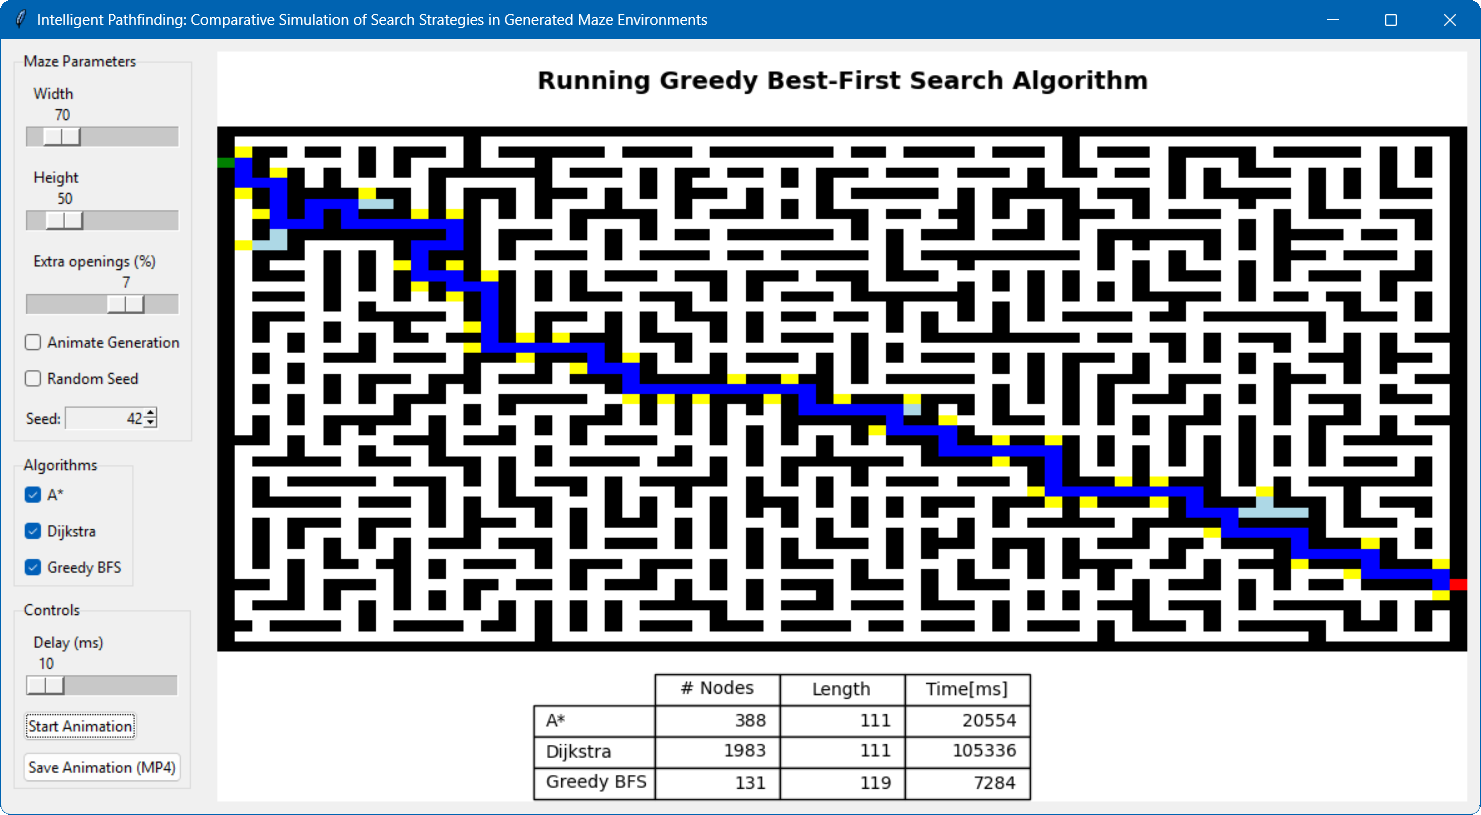
\includegraphics[width=\textwidth]{run.png}
\caption{Vergleichende Ausführung aller drei Pathfinding-Algorithmen mit Performance-Metriken}
\label{fig:algorithms}
\end{figure}

% ================== IMPLEMENTIERUNGSDETAILS ==================
\section{Implementierungsdetails}

\subsection{Architektur-Übersicht}

Die Anwendung folgt einer modularen Architektur mit klarer Trennung der Verantwortlichkeiten:

\begin{itemize}
    \item \textbf{GUI-Modul}: Benutzeroberfläche und Ereignisbehandlung
    \item \textbf{Grid-Modul}: Maze-Generierung und -Verwaltung
    \item \textbf{Search-Module}: Implementierung der Pathfinding-Algorithmen
\end{itemize}

\subsection{Performance-Optimierungen}

\subsubsection{Memory Management}
\begin{itemize}
    \item Lazy Loading durch Generatoren
    \item Effiziente NumPy-Array-Operationen
    \item Minimierung von Array-Kopien
\end{itemize}

\subsubsection{Animation-Optimierung}
\begin{itemize}
    \item Blitting für flüssige Maze-Generation
    \item Adaptive Frame-Rate basierend auf Delay-Einstellung
    \item Hintergrund-Verarbeitung für Video-Export
\end{itemize}

% ================== FAZIT ==================
\section{Fazit}

\subsection{Erreichte Ziele}

Das Projekt erfüllt alle gesetzten Ziele:
\begin{itemize}
    \item Erfolgreiche Implementierung eines robusten Maze-Generators
    \item Intuitive und funktionsreiche grafische Benutzeroberfläche
    \item Vergleichende Visualisierung von drei klassischen Pathfinding-Algorithmen
    \item Export-Funktionalität für Dokumentation
\end{itemize}

\subsection{Erkenntnisse}

\subsubsection{Algorithmische Erkenntnisse}
\begin{itemize}
    \item A* bietet den besten Kompromiss zwischen Optimalität und Effizienz
    \item Dijkstra ist unverzichtbar, wenn absolute Optimalität erforderlich ist
    \item Greedy BFS eignet sich für Echtzeit-Anwendungen mit Geschwindigkeitspriorität
\end{itemize}

\subsubsection{Technische Erkenntnisse}
\begin{itemize}
    \item Generator-Pattern ermöglicht elegante und speichereffiziente Lösungen
    \item Tkinter bleibt eine solide Wahl für GUI-Anwendungen
    \item Matplotlib-Integration erweitert Visualisierungsmöglichkeiten erheblich
\end{itemize}

\subsection{Mögliche Erweiterungen}
\begin{itemize}
    \item Bidirectional A* für noch bessere Performance
    \item Jump Point Search für Grid-optimierte Suche
    \item 3D-Maze-Generierung und -Visualisierung
    \item Verschiedene Maze-Generierungsalgorithmen (Kruskal, Prim)
    \item Interaktive Hindernis-Platzierung
    \item Multi-Agent-Pathfinding
\end{itemize}

% ================== ANHANG ==================
\newpage
\appendix

\section{Quellcode}
Github Repository: \url{https://github.com/OleMatzky/Modellierung_Endprojekt}
\begin{itemize}
    \item \href{https://github.com/OleMatzky/Modellierung_Endprojekt/blob/main/Code/gui.py}{\texttt{gui.py}} $\sim$ 500 LoC
    \item \href{https://github.com/OleMatzky/Modellierung_Endprojekt/blob/main/Code/source/grid.py}{\texttt{grid.py}} $\sim$ 120 LoC
    \item \href{https://github.com/OleMatzky/Modellierung_Endprojekt/blob/main/Code/source/search_base.py}{\texttt{search\_base.py}} $\sim$ 6 LoC
    \item \href{https://github.com/OleMatzky/Modellierung_Endprojekt/blob/main/Code/source/astar.py}{\texttt{astar.py}} $\sim$ 100 LoC
    \item \href{https://github.com/OleMatzky/Modellierung_Endprojekt/blob/main/Code/source/dijkstra.py}{\texttt{dijkstra.py}} $\sim$ 100 LoC
    \item \href{https://github.com/OleMatzky/Modellierung_Endprojekt/blob/main/Code/source/greedy.py}{\texttt{greedy.py}} $\sim$ 90 LoC
\end{itemize}

\section{Systemanforderungen}
verwendete Versionen:
\begin{itemize}
    \item Python 3.11.4
    \item NumPy 1.25
    \item Matplotlib 3.8.3
    \item Tkinter (normalerweise in Python enthalten)
    \item FFmpeg (für Video-Export, Version: 2024)
\end{itemize}

\end{document}
